\documentclass[11pt,a4paper]{article}
\usepackage[margin=19mm]{geometry}
\usepackage{amsmath,amssymb,xcolor}
\usepackage{tikz}
\usetikzlibrary{arrows.meta}
\usepackage[colorlinks=true,linkcolor=blue]{hyperref}
\definecolor{ink}{HTML}{142B50}
\definecolor{accent}{HTML}{166B8B}
\pagestyle{empty}
\setlength{\parindent}{0pt}
\setlength{\parskip}{5pt}
\newcommand{\sigmoid}{\operatorname{sigmoid}}
\begin{document}
{\LARGE\bfseries\color{ink}The learned RGB function $f(x,y)$}\par
{\small SIREN birthday greeting \enspace / \enspace 3 sine layers, width 256}
\vspace{4pt}

{\bfseries\color{accent}Network architecture}
\begin{center}
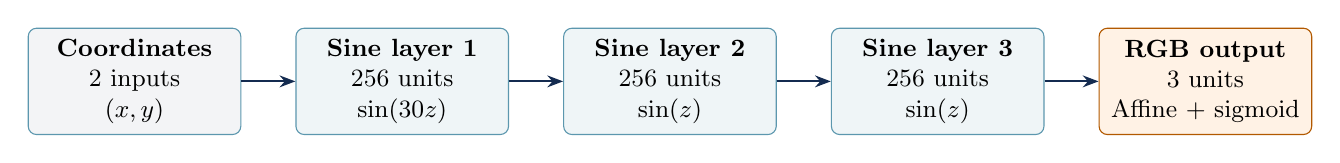
\begin{tikzpicture}[
 block/.style={draw=accent!70,fill=accent!7,rounded corners=3pt,
   minimum width=2.7cm,minimum height=1.35cm,align=center,font=\small},
 flow/.style={-{Stealth[length=2mm]},thick,draw=ink}]
\node[block,fill=ink!5] (input) at (0,0) {\textbf{Coordinates}\\2 inputs\\$(x,y)$};
\node[block] (h1) at (3.4,0) {\textbf{Sine layer 1}\\256 units\\$\sin(30z)$};
\node[block] (h2) at (6.8,0) {\textbf{Sine layer 2}\\256 units\\$\sin(z)$};
\node[block] (h3) at (10.2,0) {\textbf{Sine layer 3}\\256 units\\$\sin(z)$};
\node[block,fill=orange!10,draw=orange!70!black] (out) at (13.6,0)
 {\textbf{RGB output}\\3 units\\Affine + sigmoid};
\draw[flow] (input)--(h1);
\draw[flow] (h1)--(h2);
\draw[flow] (h2)--(h3);
\draw[flow] (h3)--(out);
\end{tikzpicture}
\end{center}
{\small All adjacent layers are fully connected; $z$ denotes each neuron's affine input.}
\vspace{4pt}

{\bfseries\color{accent}Coordinates and colour output}
\[
\begin{gathered}
\mathbf p=\begin{pmatrix}x\\y\end{pmatrix},\qquad
f(\mathbf p)=\begin{pmatrix}f_R(x,y)\\f_G(x,y)\\f_B(x,y)\end{pmatrix}\in(0,1)^3,\\[4pt]
x=\left(\frac{2(c+\tfrac12)}{640}-1\right)\frac{160}{79},
\qquad y=1-\frac{2(r+\tfrac12)}{316}.
\end{gathered}
\]
{\small $c=0,\ldots,639$ and $r=0,\ldots,315$ index image columns and rows.
The domain is $[-160/79,160/79]\times[-1,1]$; $y$ points up.}

\vspace{5pt}
{\bfseries\color{accent}Complete function in matrix form}
\[
\boxed{\begin{aligned}
\mathbf h_1&=\sin\!\left(30\left[W_1\mathbf p+\mathbf b_1\right]\right),\\
\mathbf h_2&=\sin\!\left(W_2\mathbf h_1+\mathbf b_2\right),\\
\mathbf h_3&=\sin\!\left(W_3\mathbf h_2+\mathbf b_3\right),\\
f(\mathbf p)&=\sigmoid\!\left(W_4\mathbf h_3+\mathbf b_4\right),
\qquad \sigmoid(z)=\frac{1}{1+e^{-z}}.
\end{aligned}}
\]
{\small Sine and sigmoid act on each component. The factor $30$ multiplies the
entire first affine expression, including its bias.}

\vspace{5pt}
{\bfseries\color{accent}Nested scalar form, for $C\in\{R,G,B\}$}
\[
\begin{aligned}
f_C(x,y)=\sigmoid\!\Biggl(&b_{4,C}
+\sum_{k=1}^{256}W_{4,Ck}\sin\!\Biggl[b_{3,k}
+\sum_{j=1}^{256}W_{3,kj}\sin\!\Biggl(\\[-1pt]
&b_{2,j}+\sum_{i=1}^{256}W_{2,ji}
\sin\!\Bigl(30[W_{1,i1}x+W_{1,i2}y+b_{1,i}]\Bigr)
\Biggr)\Biggr]\Biggr).
\end{aligned}
\]

\vspace{5pt}
{\bfseries\color{accent}Learned parameter dimensions}
\[
\begin{array}{c|c|c}
\text{Layer}&\text{Weight matrix}&\text{Bias vector}\\ \hline
1&W_1\in\mathbb R^{256\times2}&\mathbf b_1\in\mathbb R^{256}\\
2&W_2\in\mathbb R^{256\times256}&\mathbf b_2\in\mathbb R^{256}\\
3&W_3\in\mathbb R^{256\times256}&\mathbf b_3\in\mathbb R^{256}\\
4&W_4\in\mathbb R^{3\times256}&\mathbf b_4\in\mathbb R^{3}
\end{array}
\]
\[
\#\theta=(256\cdot2+256)
+2(256^2+256)+(3\cdot256+3)=133{,}123.
\]
{\small All $W_\ell$ and $\mathbf b_\ell$ are fixed learned values from
\texttt{colour/outputs/model.pt} (6,000 updates). This compact form represents
all coefficients symbolically; their numerical values remain in the checkpoint.}
\end{document}
